\documentclass[11pt,a4paper]{scrartcl}
\usepackage[T1]{fontenc}
\usepackage[utf8]{inputenc}
\usepackage[ngerman]{babel}
\usepackage{microtype}
\usepackage{lmodern}
\usepackage{amsmath}
\usepackage{amsfonts}
\usepackage{amssymb}
\usepackage{enumerate}
\usepackage{graphicx}

\begin{document}

\author{Gruppe 14\\Max-Emanuel Hoffmann\\Ralf Vogler\\Sebastian Wiesner}
\title{Verteilte und Web-Informationssysteme}
\subtitle{Blatt 9}

\maketitle

\section{Replikation}

\subsection{Annahmen der Herleitung des Faktors $N^3$}

Die Herleitung des Faktors $N^3$ stützt sich auf die folgenden Annahmen:

\begin{enumerate}
\item Die Anzahl der Transaktionen pro Sekunde ist für jeden Knoten konstant.
\item Jede Transaktion aktualisiert gleichverteilt eine feste Anzahl an Objekten.
\end{enumerate}

Gilt die erste Annahme nicht, so verringert sich der Faktor für die
Verklemmungsrate.  Gilt die zweite Annahme nicht, so lässt sich über den Faktor
nichts mehr aussagen, da die Anzahl der Sperren pro Transaktion nicht länger
bekannt ist.

\subsection{Herleitung des Faktors $N^3$}

\begin{align*}
  TotalEagerDeadlockRate &= TotalTransactions \times
  \frac{PD_{eager}}{TransactionDuration} = \\
  &= TotalTransactions \times \frac{PW_{eager}^2}{TotalTransactions
    \times TransactionDuration} = \\
  &= \frac{PW_{eager}^2}{TransactionDuration} = \frac{TotalTransactions^2
    \times Actions^4}{4 \times DB_{size}^2 \times TransactionDuration} = \\
  &= \frac{TPS^2 \times Actions^6 \times ActionTime^2 \times Nodes^4}{4
    \times DB_{size}^2 \times Actions \times Nodes \times ActionTime} \\
  &= \frac{TPS^2 \times Actions^5 \times ActionTime \times \mathbf{Nodes^3}}{4
    \times DB_{size}^2}
\end{align*}

Es gilt $TransactionDuration = Actions \times Nodes \times ActionTime$, da die
Aktionen einer Transaktion auf jedem Knoten ausgeführt werden müssen, bevor die
Transaktion abgeschlossen ist.  Jede Aktion benötigt dabei $ActionTime$ zur
Ausführung.

Für $TotalTransactions$ gilt $TotalTransactions = TPS \times Actions \times
ActionTime \times Nodes^2$.

Unter der Annahme, dass jede Transaktion im Mittel zur Hälfte beendet ist,
sperrt eine Transaktion $\frac{TotalTransactions \times Actions}{2}$
Ressourcen.  Da ferner alle Objekte der Datenbank gleichverteilt abgefragt
werden, ergibt sich $\frac{TotalTransactions\times Actions}{2 \times
  DB_{size}}$ als Wahrscheinlichkeit dafür, dass eine Transaktion einer von
einer anderen Transaktion gesperrte Ressource abfragt.  Jede Transaktion für
$Actions$ Aktionen durch, so dass sich für $PW_{eager}$ ergibt:

\begin{align*}
  PW_{eager} &= 1-\left(1 - \frac{TotalTransactions\times Actions}{2
      \times DB_{size}}\right)^{Actions} = \\
  &= \frac{TotalTransactions \times Actions^2}{2 \times DB_{size}}
\end{align*}

\subsection{Beispiel zur vorgeschlagenen Lösung}

Abbildung~\ref{fig:two_tier_example} zeigt ein Beispiel zur
Two-Tier-Replikation.

\begin{figure}[h]
  \centering
  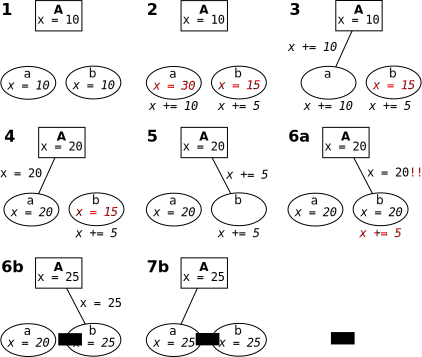
\includegraphics[width=\textwidth]{beispiel.pdf}
  \caption{Beispiel zur Two-Tier-Replikation}
  \label{fig:two_tier_example}
\end{figure}

Die Schritte des Beispiels im Einzelnen:

\begin{enumerate}
\item Ausgangssituation mit einem Basisknoten $A$ (\emph{base node}), und zwei
  mobilen Knoten (\emph{mobile nodes}) $a$ und $b$ im vollständig replizierten
  Zustand.  Die \emph{probeweisen Versionen} ((\emph{tentative version})) der
  mobilen Knoten sind in kursiver Schrift dargestellt, die \emph{Hauptversion}
  (\emph{master version}) in normaler Schrift.  Der Basisknoten $A$ ist der
  Hauptknoten (\emph{master node}) für das Objekt $x$.
\item Die beiden mobilen Knoten aktualisieren ihre lokalen Versionen mit
  unterschiedlichen \emph{probeweisen Transaktionen} (\emph{tentative
    transactions}).  Die veränderten, nicht replizierten Daten sind in roter
  Schrift dargestellt, die dazugehörige Transaktion ist unter dem
  entsprechenden mobilen Knoten gezeigt.
\item Der mobile Knoten $a$ verbindet sich mit dem Basisknoten, verwirft seine
  probeweisen Versionen der Daten und sendet die noch nicht replizierten
  Transaktionen.
\item Der Basisknoten führt die empfangene Transaktion als
  \emph{Basistransaktion} (\emph{base transaction}) durch, und sendet die
  aktualisierte Hauptversion (\emph{master version}) der Daten an den mobilen
  Knoten, der seine lokalen Daten entsprechend aktualisiert und die Verbindung
  anschließend trennt.
\item Der mobile Knoten $b$ verbindet sich mit dem Masterknoten und beginnt nun
  seinerseits die Replizierung entsprechend Schritt~3.
\end{enumerate}

Im Folgenden zeigt das Beispiel den Fortgang mit zwei verschiedenen
Akzeptanzkriterien für durchgeführte Transaktionen.  In Teil~a gilt das starke
Akzeptanzkriterium, dass die Basistransaktion \emph{exakt dasselbe} Ergebnis
zur Folge haben muss wie die im mobilen Knoten zuvor durchgeführte probeweise
Transaktion.  Mithin schlägt die Basistransaktion in Schritt~6a fehlt
(angezeigt durch die zwei Ausrufezeichen in roter Schritt), der mobile Knoten
$b$ erhält die aktuelle Hauptversion des Datums und zeigt dem Nutzer im
folgenden den Fehlschlag der Transaktion an.  Die fehlgeschlagene Transaktion
ist in roter Farbe markiert.

In Teil~b gilt dagegen das schwächere Akzeptanzkriterium, dass der Wert von $x$
nicht negativ werden kann.  Mithin wird die Transaktion in Schritt~6b
erfolgreich durchgeführt, und die Replizierung verläuft analog zu Schritt~4.
7b zeigt anschließend noch, wie sich der Knoten $a$ im Anschluss erneut
verbindet und die nun aktuelle Hauptversion des Datums erhält.

\end{document}
